\documentclass[pdf,sprung,slideColor,nocolorBG]{beamer}
%
%\documentclass[hyperref={pdfpagelabels=false}]{beamer}
\mode<presentation>

\newenvironment{colortheme}[1]{
\def\ProvidesPackageRCS $##1${\relax}
\renewcommand{\ProcessOptions}{\relax}
\makeatletter
\input beamercolortheme#1.sty
\makeatother
}{}

\let\Tiny=\tiny
\usetheme{Adelaide}
\usefonttheme[stillsansseriftext]{serif}
\setbeamerfont{structure}{series=\bfseries}
\setbeamertemplate{frametitle}[default][center]
\usepackage[figurename={}]{caption}
\usepackage[latin1]{inputenc}
%\usepackage{amsmath}   %needed for \begin{align}... \end{align} environment
\usepackage{amsfonts}
\usepackage{amssymb}
\usepackage{amscd}
\usepackage[all]{xy}
\usepackage{xcolor}
\usepackage{enumerate}
%
\newcommand{\slidecite}[1]{\tiny{(#1)}\normalsize{}}
\newcommand{\smallcite}[1]{\small{(#1)}\normalsize{}}

\newcommand{\mb}[1]{\mathbb{#1}}
\newcommand{\mf}[1]{\mathbf{#1}}
\newcommand{\Emph}[1]{\emph{\textcolor{blue}{#1}}}

\newcommand{\abs}[1]{\left| #1 \right|}
\newcommand{\norm}[1]{\left\| #1 \right\|}
\newcommand{\To}{\rightarrow}

\newcommand{\Cay}[1]{\operatorname{Cay}\left(#1\right)}
\newcommand{\Clique}[1]{\omega\left(#1\right)}
\newcommand{\dual}[1]{\widetilde{#1}}
\newcommand{\support}[1]{\operatorname{supp}\left(#1\right)}
\newcommand{\weight}[1]{\operatorname{wt}\left(#1\right)}
\newcommand{\weightclass}[1]{\operatorname{wc}\left(#1\right)}

\newcommand{\G}{\mb{G}}
\newcommand{\R}{\mb{R}}
\newcommand{\Z}{\mb{Z}}
%\newtheorem{Definition}{Definition}
\newtheorem{Conjecture}{Conjecture}
\newtheorem{Question}{Question}
\newtheorem{Proposition}{Proposition}

\title{Classifying bent functions by their Cayley graphs, using Sage}
\author{Paul Leopardi}

\date{DRAFT ONLY
\\
For RMIT University Melbourne 2017}

\institute{Australian Government - Bureau of Meteorology
\\
University of Melbourne}
\titlegraphic{
%\includegraphics[angle=0,width=10mm]{../../common/beamer-anu-colourlogo.png}
%\includegraphics[angle=0,width=20mm]{../../common/carma_logo.jpg}
}
\begin{document}

\frame{\titlepage}
\begin{frame}
\frametitle{Acknowledgements}
\begin{center}
~

Nathan Clisby,
Robert Craigen,
Joanne Hall,
David Joyner, Philippe Langevin, William Martin,
Padraig {\'O} Cath{\'a}in,
Judy-anne Osborn, Dima Pasechnik and William Stein.

~

kodlu on MathOverflow.

~

Matthew Leingang for Beamer colour themes.

~

Australian National University. University of Newcastle, Australia. University of Melbourne.

~

SageMath, Bliss, Nauty.

~

Australian Government - Bureau of Meteorology.
\end{center}
\end{frame}

\begin{frame}
\frametitle{Overview}
%\begin{center}
\begin{itemize}
\item
Key concepts.

~

\item
Equivalence.

~

\item
Some results.

~

\item
Observations for small dimensions.

~

\item
Some questions.

~

\item
SageMath code.
\end{itemize}

%\end{center}
\end{frame}

\section{Key concepts}
\begin{colortheme}{seagull}
\begin{frame}
\frametitle{Bent functions}
% Bent functions can be defined in a number of equivalent ways.
% The definition used here involves the Walsh Hadamard Transform.
\begin{Definition}
\label{def-Walsh-Hadamard-transform}
The Walsh Hadamard transform of
a Boolean function $f : \Z_2^m \To \Z_2$ is
\begin{align*}
W_f(y)
&:=
\sum_{x \in \Z_2^{2 m}} (-1)^{\langle x, y \rangle} + f(x)
\end{align*}
\end{Definition}

\begin{Definition}
\label{def-Bent-function}
A Boolean function $f : \Z_2^m \To \Z_2$ is \Emph{bent}
if and only if its Walsh Hada\-mard transform has constant magnitude $2^{-m}$.
% \cite[p. 74]{Dil74}
% \cite[p. 300]{Rot76}.
\end{Definition}
\slidecite{Dillon 1974; Rothaus 1976}
\end{frame}
\begin{frame}
\frametitle{Dual bent functions}

\begin{Definition}
\label{def-dual-Bent-function}
For a bent function $f$, the function $\dual{f}$, defined by
\begin{align*}
(-1)^{\dual{f}(x)} &:= 2^{-m} \sum_{y \in \Z_2^{2m}} (-1)^{f(y) + \langle x, y \rangle}
\end{align*}
is called the \Emph{dual} of $f$.
\end{Definition}

~

The function $\dual{f}$ is also a bent function on $\Z_2^{2m}$.

~

\slidecite{Dillon 1974; Rothaus 1976; Tokareva 2011}
\end{frame}

\begin{colortheme}{jubata}
\begin{frame}
\frametitle{Weights and weight classes}
\begin{Definition}
The \Emph{weight} of a binary function is the cardinality of its \Emph{support}.
For $f$ on $\Z_2^{2m}$
\begin{align*}
\support{f} &:= \{x \in \Z_2^{2m} \mid f(x)=1 \}.
\end{align*}

A bent function $f$ on $\Z_2^{2m}$ has weight
\begin{align*}
\weight{f} &= 2^{2 m - 1} - 2^{m-1} \quad (\text{weight class~} \weightclass{f}=0), \text{~or}
\\
\weight{f} &= 2^{2 m - 1} + 2^{m-1} \quad (\text{weight class~} \weightclass{f}=1).
\end{align*}
% If $f(0)=0$ then $\weightclass{\Cay{f}} := \weightclass{f}$.
\end{Definition}
\end{frame}
\end{colortheme}

\begin{frame}
\frametitle{The Cayley graph of a Boolean function}
%\begin{center}
The \Emph{Cayley graph} $\Cay{f}$ of a Boolean function

~

\begin{align*}
%
f : \Z_2^n \To \Z_2 \quad \text{where} \quad f(0) = 0
%
\end{align*}

~

is
an undirected graph with

\begin{align*}
V(\Cay{f}) &:= \Z_2^n, \quad (x,y) \in E(\Cay{f}) \Leftrightarrow f(x+y) = 1.
\end{align*}

~

\slidecite{Bernasconi and Codenotti 1999}
\end{frame}

\begin{frame}
\frametitle{Strongly regular graphs}
%\begin{center}
A simple graph $\Gamma$ of order $v$ is \Emph{strongly regular} with parameters
$(v,k,\lambda,\mu)$ if

~

\begin{itemize}
 \item
each vertex has degree $k,$

~
 \item
each adjacent pair of vertices has $\lambda$ common neighbours, and

~
\item
each nonadjacent pair of vertices has $\mu$ common neighbours.
\end{itemize}

~

\slidecite{Brouwer, Cohen and Neumaier 1989}

%\end{center}
\end{frame}

\begin{frame}
\frametitle{Bent functions and strongly regular graphs}

\begin{Proposition}
\smallcite{Bernasconi and Codenotti 1999}

The Cayley graph $\Cay{f}$ of a bent function $f$ on $\Z_2^{2m}$

with $f(0)=0$ is a strongly regular graph with $\lambda = \mu.$
\end{Proposition}

The parameters of $\Cay{f}$ are
\begin{align*}
(v,k,\lambda) = &(4^m, 2^{2 m - 1} - 2^{m-1}, 2^{2 m - 2} - 2^{m-1})
\\
  \text{or} \quad &(4^m, 2^{2 m - 1} + 2^{m-1}, 2^{2 m - 2} + 2^{m-1}).
\end{align*}

~

\slidecite{Menon 1962; Dillon 1974; Bernasconi and Codenotti 1999}
%\end{center}
\end{frame}
\end{colortheme}
\begin{colortheme}{seagull}
\begin{frame}
\frametitle{Projective two-weight binary codes}

\begin{Definition}
A \Emph{two-weight binary code} with parameters $[n,k,d]$ is a $k$ dimensional subspace of $\Z_2^n$ with
minimum Hamming distance $d$, such that the set of Hamming weights of the non-zero vectors has size 2.

~

``A \Emph{generator matrix} $G$ of a linear code $[n, k]$ code $C$ is any matrix
of rank $k$ (over $\Z_2$) with rows from $C.$''

~

``A linear $[n, k]$ code is called \Emph{projective} if no two columns of a generator matrix
$G$ are linearly dependent, i.e., if the columns of $G$ are pairwise different points in a
projective $(k-1)$-dimensional space.''
In the case of $\Z_2$, no two columns are equal.

~

\end{Definition}

\slidecite{Tonchev 1996; Bouyukliev, Fack, Willems and Winne 2006}

\end{frame}
\end{colortheme}

\begin{colortheme}{seagull}
\begin{frame}
\frametitle{From bent function to linear code (1)}
\begin{Definition}

\smallcite{Carlet 2007; Ding 2015, Corollary 10}

For a bent function $f : \Z_2^{2m} \To \Z_2$,
define the linear code $C(f)$ by the generator matrix
\begin{align*}
M C(f)_{x,y} &\in \Z_2^{4^m \times \weight{f}},
\\
M C(f)_{x,y} &:= \langle x, \support{f}(y) \rangle,
\end{align*}
with $x$ in lexicographic order of $\Z_2^{2m}$
and $\support{f}(y)$ in lexicographic order of $\support{f}$.

The $4^m$ words of the code $C(f)$ are the rows of the generator matrix $M C(f)$.
\end{Definition}

\slidecite{Carlet 2007; Ding 2015, Corollary 10}

\end{frame}
\begin{frame}
\frametitle{From bent function to linear code (2)}
\begin{Theorem}
\smallcite{Carlet 2007, Prop. 20; Ding 2015, Corollary 10}

For a bent function $f : \Z_2^{2m} \To \Z_2$, the linear code $C(f)$
is a two-weight projective binary code.

~

The possible weights of non-zero code words are:
\begin{align*}
\begin{cases}
2^{2m-2}, 2^{2m-2} - 2^{m-1} & \text{if~} \weightclass{f}=0.
\\
2^{2m-2}, 2^{2m-2} + 2^{m-1} & \text{if~} \weightclass{f}=1.
\end{cases}
\end{align*}

\end{Theorem}

\slidecite{Carlet 2007, Prop. 20; Ding 2015, Corollary 10}

\end{frame}
\begin{frame}
\frametitle{From linear code to strongly regular graph}
\begin{Definition}
\label{R-f-def}
Given $f : \Z_2^{2m} \To \Z_2$, form the linear code $C(f)$.

The graph $R(f)$ is defined as:

Vertices of $R(f)$ are code words of $C(f)$.

For $v,w \in C(f)$, edge $(u,v) \in R(f)$ if and only if
\begin{align*}
\begin{cases}
\weight{u+v} = 2^{2m-2} - 2^{m-1} & (\weightclass{f}=0).
\\
\weight{u+v} = 2^{2m-2} + 2^{m-1} & (\weightclass{f}=1).
\end{cases}
\end{align*}

\end{Definition}
Since $C(f)$ is a two-weight binary projective code,
$R(f)$ is a strongly regular graph.

\slidecite{Delsarte 1972, Theorem 2}
\end{frame}
\begin{frame}
\frametitle{The two block designs of a bent function}

The first block design of a bent function $f$ is obtained by interpreting
the adjacency matrix of $\Cay{f}$ as the incidence matrix of a block design.
In this case we do not need $f(0)=0$.

~
\begin{Definition}
The second block design of a bent function $f$ is defined by the incidence matrix
$D(f)$ where
\begin{align*}
D(f)_{c,x} &:= f(x) + \langle c, x \rangle + \dual{f}(c).
\end{align*}
This is a symmetric block design with the \Emph{symmetric difference property},
called the \Emph{SDP design} of $f$.
\end{Definition}

~

\slidecite{Kantor 1983; Dillon and Schatz 1987; Neumann 2006}
\end{frame}
\end{colortheme}

\section{Equivalence}

\begin{colortheme}{seagull}
\begin{frame}
\frametitle{Extended affine equivalence}

\begin{Definition}
For bent functions $f,g : \Z_2^{2m} \To \Z_2$,

$f$ is \Emph{extended affine equivalent} to $g$ if and only if
\begin{align*}
g(x) &= f(A x + b) + \langle c, x \rangle + \delta
\end{align*}
for some $A \in GL(2m,2)$, $b, c \in \Z_2^{2m}$, $\delta \in \Z_2$.
\end{Definition}
~

\slidecite{Tokareva 2014}
\end{frame}
\begin{frame}
\frametitle{General linear equivalence}

\begin{Definition}
For bent functions $f,g : \Z_2^{2m} \To \Z_2$,
$f$ is \Emph{general linear equivalent} to $g$ if and only if
\begin{align*}
g(x) &= f(A x)
\end{align*}
for some $A \in GL(2m,2)$.
\end{Definition}
\end{frame}
\end{colortheme}

\begin{colortheme}{jubata}
\begin{frame}
\frametitle{Extended translation equivalence}

\begin{Definition}
For bent functions $f,g : \Z_2^{2m} \To \Z_2$,

$f$ is \Emph{extended translation equivalent} to $g$ if and only if
\begin{align*}
g(x) &= f(x + b) + \langle c, x \rangle + \delta
\end{align*}
for $b, c \in \Z_2^{2m}$, $\delta \in \Z_2$.
\end{Definition}
\end{frame}
\end{colortheme}

\begin{colortheme}{jubata}
\begin{frame}
\frametitle{Cayley equivalence}
\begin{Definition}
%
For $f, g : \Z_2^{2m} \To \Z_2$, with both $f$ and $g$ bent,

we call $f$ and $g$ \Emph{Cayley equivalent},
and write $f \equiv g$,

if and only if $f(0)=g(0)=0$ and $\Cay{f} \equiv \Cay{g}$ as graphs.

~

Equivalently, $f \equiv g$ if and only if $f(0)=g(0)=0$ and

there exists a bijection $\pi : \Z_2^{2m} \To \Z_2^{2m}$ such that
\begin{align*}
g(x+y) &= f \big(\pi(x)+\pi(y)\big) \quad \text{for all~} x,y \in \Z_2^{2m}.
\end{align*}
\end{Definition}
\end{frame}
\begin{frame}
\frametitle{Extended Cayley equivalence}
\begin{Definition}
For $f, g : \Z_2^{2m} \To \Z_2$, with both $f$ and $g$ bent,

if there exist $\delta, \epsilon \in \{0,1\}$ such that $f + \delta \equiv g + \epsilon$,

we call $f$ and $g$ \Emph{extended Cayley (EC) equivalent} and write $f \cong g$.
\end{Definition}
Extended Cayley equivalence is an equivalence relation on the set of all bent functions on $\Z_2^{2m}$.
\end{frame}
\section{Some results}

\begin{frame}
\frametitle{Linear equivalence implies Cayley equivalence}

\begin{Theorem}
If $f$ is bent with $f(0)=0$ and $g(x) := f(A x)$ where $A \in GL(2m,2)$,
then $g$ is bent with $g(0)=0$ and $f \equiv g$.
\end{Theorem}
\begin{proof}
\begin{align*}
g(x+y) &= f\big(A(x+y)\big) = f(A x + A y)\quad \text{for all~} x,y \in \Z_2^{2m}.
\end{align*}
\end{proof}

\end{frame}

\begin{frame}
\frametitle{Extended affine, extended translation and extended Cayley equivalence (1)}

\begin{Theorem}
For $A \in GL(2m,2)$, $b, c \in \Z_2^{2m}$, $\delta \in \Z_2$,
$f : \Z_2^{2m} \To \Z_2$,

the function
\begin{align*}
h(x) &:= f(A x + b) + \langle c, x \rangle + \delta
\intertext{can be expressed as $h(x) = g(A x)$ where}
g(x) &:= f(x+b) + \langle (A^{-1})^T c, x \rangle + \delta,
\end{align*}
and therefore if $f$ is bent then $h \cong g$.
\end{Theorem}
\end{frame}

\begin{frame}
\frametitle{Extended affine, extended translation and extended Cayley equivalence (2)}

Therefore, to determine the extended Cayley equivalence classes within the extended affine equivalence class of
a bent function $f : \Z_2^{2m} \To \Z_2$, for which $f(0)=0$, we need only examine
the extended translation equivalent functions of the form
\begin{align*}
f(x+b) + \langle c, x \rangle + f(b),
\end{align*}
for each $b, c \in \Z_2^{2m}$.
\end{frame}
\begin{frame}
\frametitle{Quadratic bent functions have 2 EC classes}
\begin{Theorem}
For each $m>0$, the extended affine equivalence class of quadratic bent functions
$q : \Z_2^{2m} \To \Z_2$ contains exactly two extended Cayley equivalence classes,
corresponding to the two possible weight classes of $x \mapsto q(x+b) + \langle c, x \rangle + q(b)$.
\end{Theorem}

\end{frame}
%\end{colortheme}

%\begin{colortheme}{jubata}
\begin{frame}
\frametitle{The strongly regular graph $R(f)$ \\ is the Cayley graph of the dual}

\begin{Theorem}
For $f : \Z_2^{2m} \To \Z_2$, with $f(0)=0$,
\begin{align*}
R(f) &\equiv \Cay{\dual{f} + \weightclass{f}}.
\end{align*}
\end{Theorem}

\end{frame}
\begin{frame}
\frametitle{The SDP design matrix}
\begin{Theorem}
For every bent function $f$, the \Emph{weight class matrix} of $f$
equals the incidence matrix of the SDP design of $f$.

~

Specifically,
\begin{align*}
\weightclass{\Cay{x \mapsto f(x+b) + \langle c, x \rangle + f(b)}}
&=
f(b) + \langle c, b \rangle + \dual{f}(c)
\\
&=
D(f)_{c,b}.
\end{align*}

\end{Theorem}

\end{frame}
\end{colortheme}
\section{Observations}
\begin{colortheme}{jubata}
\begin{frame}
\frametitle{For 2 dimensions: classes}

One extended affine class, containing the extended translation class $[f_{2,1}]$,
where $f_{2,1}(x) := x_0 x_1$ is self dual.

~

Two extended Cayley classes:
\begin{align*}
\begin{array}{|cccl|}
\hline
\text{Class} &
\text{Parameters} &
\text{2-rank} &
\text{Clique polynomial}
\\
\hline
1 &
(4, 1, 0, 0) & 4 &
2t^{2} + 4t + 1
\\
2 &
K_4 & 4 &
t^{4} + 4t^{3} + 6t^{2} + 4t + 1
\\
\hline
\end{array}
\end{align*}

\end{frame}
\begin{frame}
\frametitle{For ET class $[f_{2,1}]$: matrices}
\begin{figure}
\centering
\begin{minipage}{.48\textwidth}
  \centering
  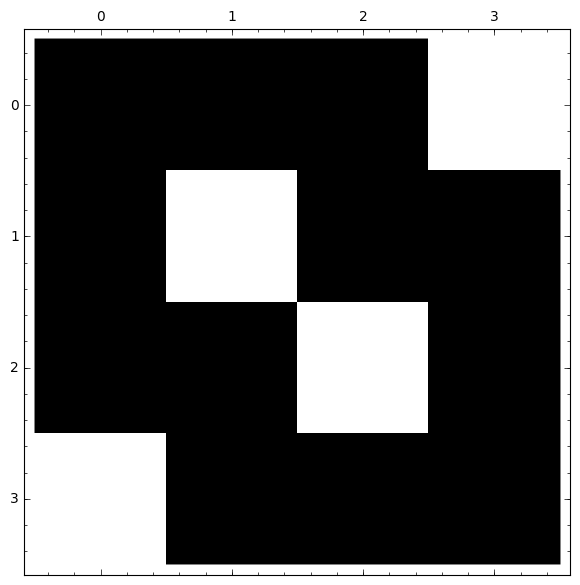
\includegraphics[width=.9\linewidth]{../matrix_plot/re2_1_weight_class_matrix.png}
  \captionof{figure}{$[f_{2,1}]$: weight classes}
  \label{fig:c2_1_weight_class_matrix}
\end{minipage}%
\begin{minipage}{.48\textwidth}
  \centering
  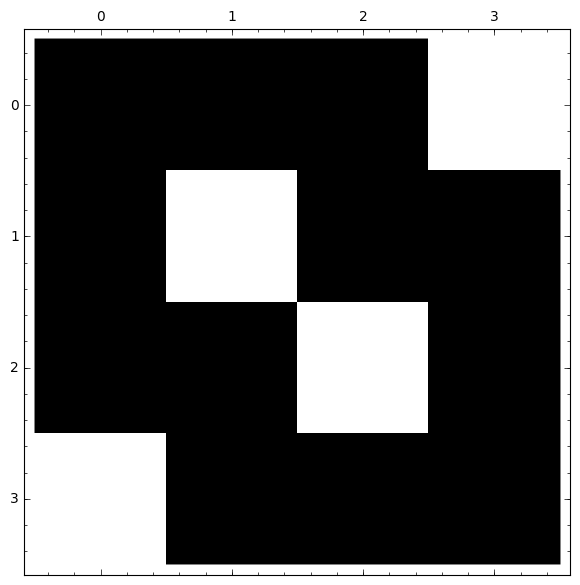
\includegraphics[width=.9\linewidth]{../matrix_plot/re2_1_bent_cayley_graph_index_matrix.png}
  \captionof{figure}{$[f_{2,1}]$: extended Cayley classes}
  \label{fig:c2_1_bent_cayley_graph_index_matrix}
\end{minipage}
\end{figure}
\end{frame}
\begin{frame}
\frametitle{For 4 dimensions: classes}

One extended affine class, containing the extended translation class $[f_{4,1}]$, where
$f_{4,1}(x) := x_0 x_1 + x_2 x_3$ is self dual.

~

Two extended Cayley classes:
\begin{align*}
\begin{array}{|cccl|}
\hline
\text{Class} &
\text{Parameters} &
\text{2-rank} &
\text{Clique polynomial}
\\
\hline
1 &
(16, 6, 2, 2) &
6 &
8t^{4} + 32t^{3} + 48t^{2} + 16t + 1
\\
2 &
(16, 10, 6, 6) &
6 &
\begin{array}{l}
16t^{5} + 120t^{4} + 160t^{3} +
\\
80t^{2} + 16t + 1
\end{array}
\\
\hline
\end{array}
\end{align*}
\end{frame}
\begin{frame}
\frametitle{For ET class $[f_{4,1}]$: matrices}
\begin{figure}
\centering
\begin{minipage}{.48\textwidth}
  \centering
  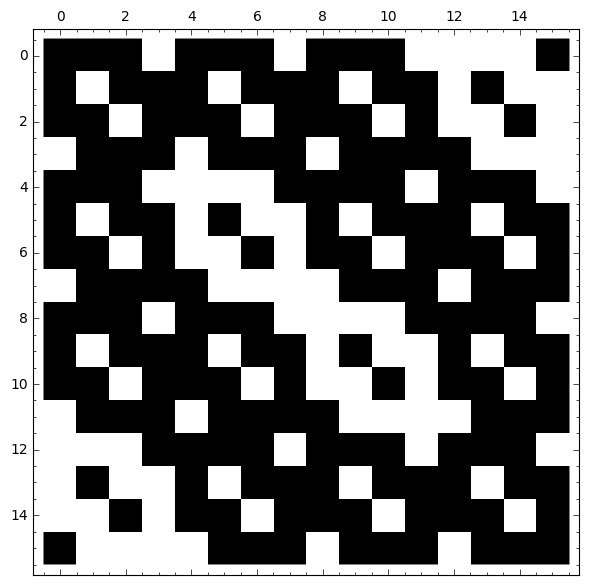
\includegraphics[width=.9\linewidth]{../matrix_plot/re4_1_weight_class_matrix.png}
  \captionof{figure}{$[f_{4,1}]$: weight classes}
  \label{fig:c4_1_weight_class_matrix}
\end{minipage}%
\begin{minipage}{.48\textwidth}
  \centering
  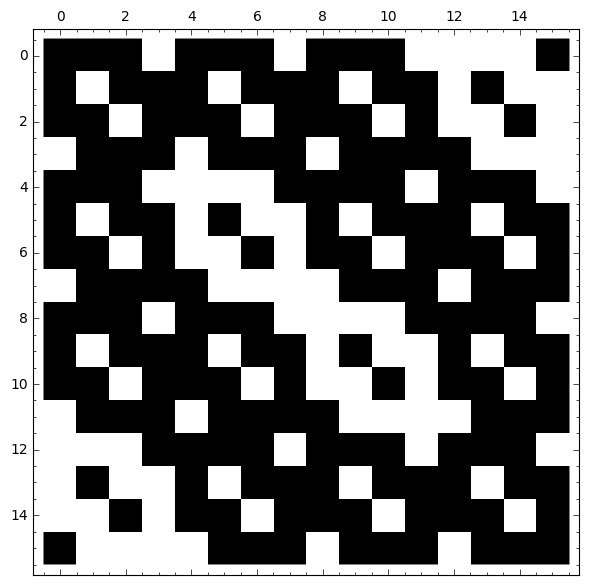
\includegraphics[width=.9\linewidth]{../matrix_plot/re4_1_bent_cayley_graph_index_matrix.png}
  \captionof{figure}{$[f_{4,1}]$: extended Cayley classes}
  \label{fig:c4_1_bent_cayley_graph_index_matrix}
\end{minipage}
\end{figure}
\end{frame}
\begin{frame}
\frametitle{For 6 dimensions: ET classes}

Four extended affine classes, containing the following extended translation classes:

\begin{align*}
\def\arraystretch{1.2}
\begin{array}{|cl|}
\hline
\text{Class} &
\text{Representative}
\\
\hline
\,[f_{6,1}] & f_{6,1} :=
\begin{array}{l}
x_{0} x_{1} + x_{2} x_{3} + x_{4} x_{5}
\end{array}
\\
\,[f_{6,2}] & f_{6,2} :=
\begin{array}{l}
x_{0} x_{1} x_{2} + x_{0} x_{3} + x_{1} x_{4} + x_{2} x_{5}
\end{array}
\\
\,[f_{6,3}] & f_{6,3} :=
\begin{array}{l}
x_{0} x_{1} x_{2} + x_{0} x_{1} + x_{0} x_{3} + x_{1} x_{3} x_{4} + x_{1} x_{5}
\\
 +\, x_{2} x_{4} + x_{3} x_{4}
\end{array}
\\
\,[f_{6,4}] & f_{6,4} :=
\begin{array}{l}
x_{0} x_{1} x_{2} + x_{0} x_{3} + x_{1} x_{3} x_{4} + x_{1} x_{5} + x_{2} x_{3} x_{5}
\\
 +\, x_{2} x_{3} + x_{2} x_{4} + x_{2} x_{5} + x_{3} x_{4} + x_{3} x_{5}
\end{array}
\\
\hline
\end{array}
\end{align*}
\end{frame}
\begin{frame}
\frametitle{For ET class $[f_{6,1}]$: EC classes}

Bent function
$f_{6,1}(x) = x_0 x_1 + x_2 x_3 + x_4 x_5$ is self dual.

 ~

Two extended Cayley classes corresponding to Tonchev's two-weight projective codes:
\begin{align*}
\def\arraystretch{1.2}
\begin{array}{|ccl|}
\hline
\text{Class} &
\text{Parameters} & \text{Reference}
\\
\hline
0 & [35,6,16] & \text{Table 1.156 1, 2 (complement)}
\\
1 & [27,6,12] & \text{Table 1.155 1 }
\\
\hline
\end{array}
\end{align*}

Graph for class 0 is also isomorphic to the complement of Royle's $(64,35,18,20)$ strongly regular
graph $X$.

\slidecite{Tonchev 1996, 2006; Royle 2008}
 \end{frame}
\begin{frame}
\frametitle{For ET class $[f_{6,1}]$: matrices}
\begin{figure}
\centering
\begin{minipage}{.48\textwidth}
  \centering
  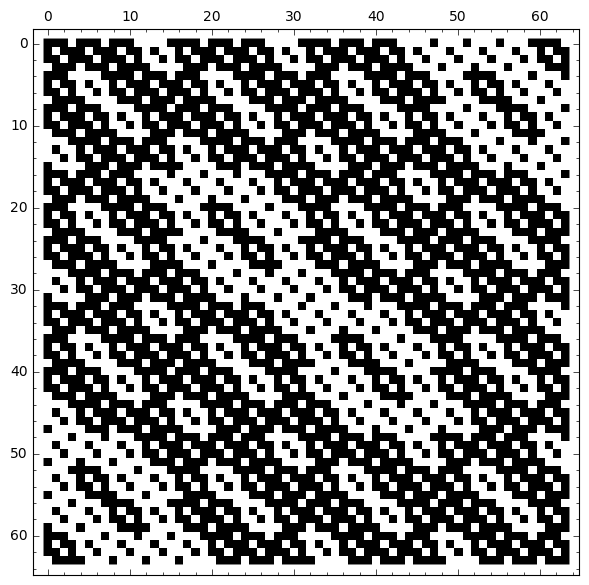
\includegraphics[width=.9\linewidth]{../matrix_plot/re6_1_weight_class_matrix.png}
  \captionof{figure}{$[f_{6,1}]$: weight classes}
  \label{fig:6_1_weight_class_matrix}
\end{minipage}%
\begin{minipage}{.48\textwidth}
  \centering
  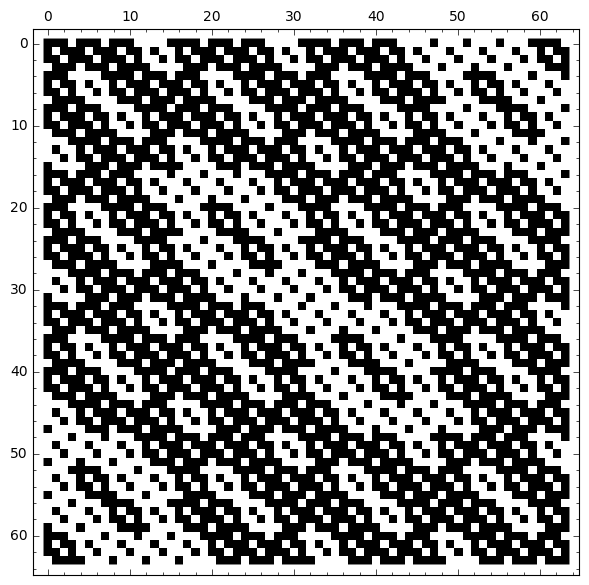
\includegraphics[width=.9\linewidth]{../matrix_plot/re6_1_bent_cayley_graph_index_matrix.png}
  \captionof{figure}{$[f_{6,1}]$: 2 extended Cayley classes}
  \label{fig:6_1_bent_cayley_graph_index_matrix}
\end{minipage}
\end{figure}
\end{frame}
\begin{frame}
\frametitle{For ET class $[f_{6,2}]$: EC classes}

Bent function
$f_{6,2}(x) = x_{0} x_{1} x_{2} + x_{0} x_{3} + x_{1} x_{4} + x_{2} x_{5}$.

~

Three extended Cayley classes corresponding to Tonchev's two-weight projective codes:
\begin{align*}
\def\arraystretch{1.2}
\begin{array}{|ccl|}
\hline
\text{Class} &
\text{Parameters} & \text{Reference}
\\
\hline
0 & [35,6,16] & \text{Table 1.156 1, 2 (complement)}
\\
1 & [35,6,16] & \text{Table 1.156 3 (complement)}
\\
2 & [27,6,12] & \text{Table 1.155 2 }
\\
\hline
\end{array}
\end{align*}

Graph for class 0 is also isomorphic to that of $[f_{6,1}]$ class 0.

\slidecite{Tonchev 1996, 2006}
\end{frame}
\begin{frame}
\frametitle{For ET class $[f_{6,2}]$: matrices}
\begin{figure}
\centering
\begin{minipage}{.48\textwidth}
  \centering
  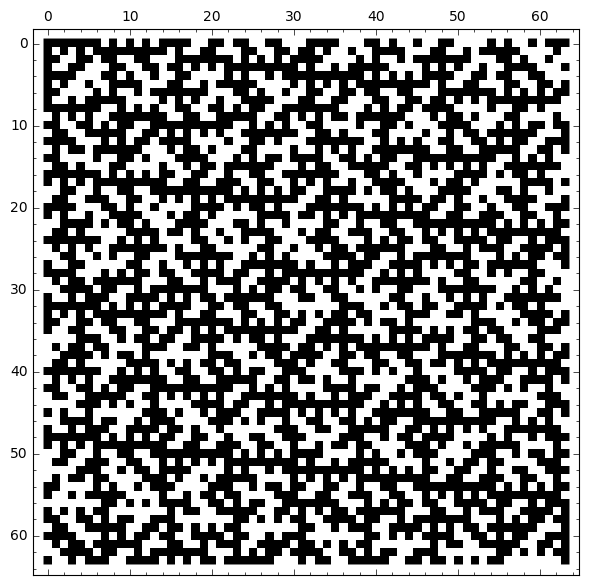
\includegraphics[width=.9\linewidth]{../matrix_plot/re6_2_weight_class_matrix.png}
  \captionof{figure}{$[f_{6,2}]$: weight classes}
  \label{fig:6_2_weight_class_matrix}
\end{minipage}%
\begin{minipage}{.48\textwidth}
  \centering
  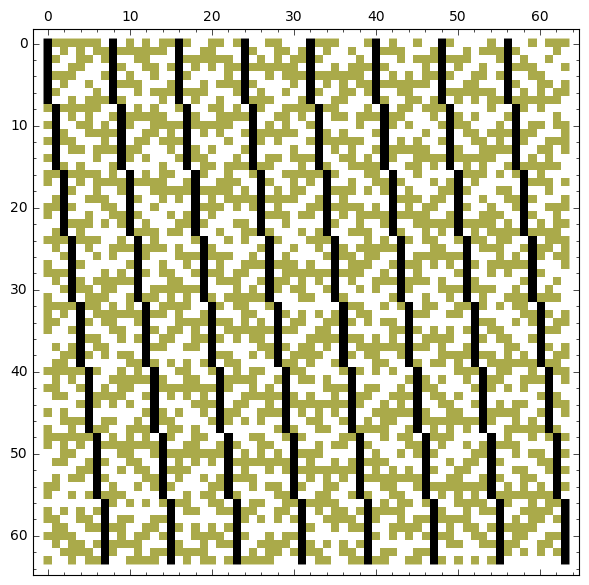
\includegraphics[width=.9\linewidth]{../matrix_plot/re6_2_bent_cayley_graph_index_matrix.png}
  \captionof{figure}{$[f_{6,2}]$: 3 extended Cayley classes}
  \label{fig:6_2_bent_cayley_graph_index_matrix}
\end{minipage}
\end{figure}
\end{frame}
\begin{frame}
\frametitle{For ET class $[f_{6,3}]$: EC classes}

Bent function
\begin{align*}
f_{6,3}(x) &= x_{0} x_{1} x_{2} + x_{0} x_{1} + x_{0} x_{3} + x_{1} x_{3} x_{4}
\\
           &+ x_{1} x_{5} + x_{2} x_{4} + x_{3} x_{4}.
\end{align*}

Four extended Cayley classes corresponding to Tonchev's two-weight projective codes:
\begin{align*}
\def\arraystretch{1.2}
\begin{array}{|ccl|}
\hline
\text{Class} &
\text{Parameters} & \text{Reference}
\\
\hline
0 & [35,6,16] & \text{Table 1.156 4 (complement)}
\\
1 & [27,6,12] & \text{Table 1.155 3 }
\\
2 & [35,6,16] & \text{Table 1.156 5 (complement)}
\\
3 & [27,6,12] & \text{Table 1.155 4 }
\\
\hline
\end{array}
\end{align*}

\slidecite{Tonchev 1996, 2006}
\end{frame}
\begin{frame}
\frametitle{For ET class $[f_{6,3}]$: matrices}
\begin{figure}
\centering
\begin{minipage}{.48\textwidth}
  \centering
  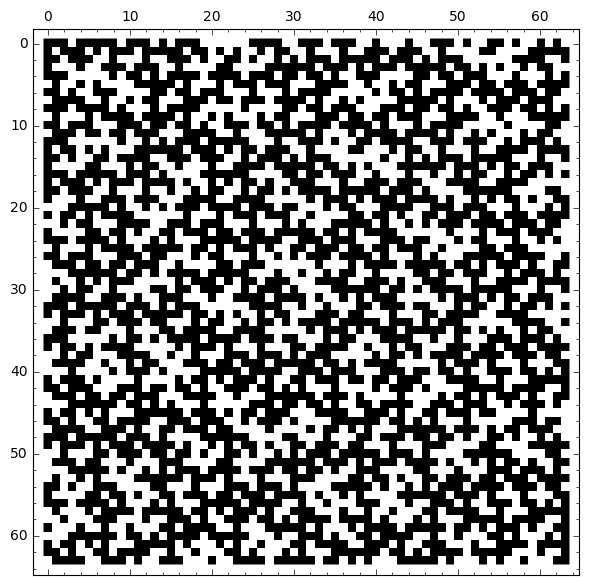
\includegraphics[width=.9\linewidth]{../matrix_plot/re6_3_weight_class_matrix.png}
  \captionof{figure}{$[f_{6,3}]$: weight classes}
  \label{fig:6_3_weight_class_matrix}
\end{minipage}%
\begin{minipage}{.48\textwidth}
  \centering
  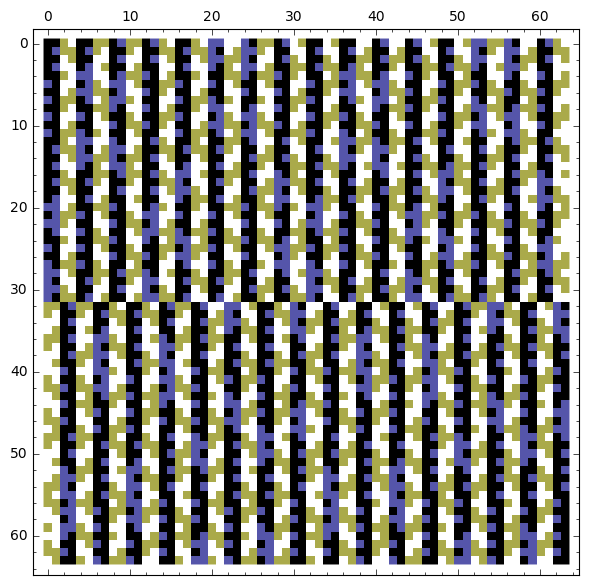
\includegraphics[width=.9\linewidth]{../matrix_plot/re6_3_bent_cayley_graph_index_matrix.png}
  \captionof{figure}{$[f_{6,3}]$: 4 extended Cayley classes}
  \label{fig:6_3_bent_cayley_graph_index_matrix}
\end{minipage}
\end{figure}
\end{frame}
\begin{frame}
\frametitle{For ET class $[f_{6,4}]$: EC classes}

Bent function
\begin{align*}
f_{6,4}(x) &= x_{0} x_{1} x_{2} + x_{0} x_{3} + x_{1} x_{3} x_{4} + x_{1} x_{5} + x_{2} x_{3} x_{5}
\\
           &+ x_{2} x_{3} + x_{2} x_{4} + x_{2} x_{5} + x_{3} x_{4} + x_{3} x_{5}.
\end{align*}

Three extended Cayley classes corresponding to Tonchev's two-weight projective codes:
\begin{align*}
\def\arraystretch{1.2}
\begin{array}{|ccl|}
\hline
\text{Class} &
\text{Parameters} & \text{Reference}
\\
\hline
0 & [35,6,16] & \text{Table 1.156 7 (complement)}
\\
1 & [35,6,16] & \text{Table 1.156 6 (complement)}
\\
2 & [27,6,12] & \text{Table 1.155 5 }
\\
\hline
\end{array}
\end{align*}

\slidecite{Tonchev 1996, 2006}
\end{frame}
\begin{frame}
\frametitle{For ET class $[f_{6,4}]$: matrices}
\begin{figure}
\centering
\begin{minipage}{.48\textwidth}
  \centering
  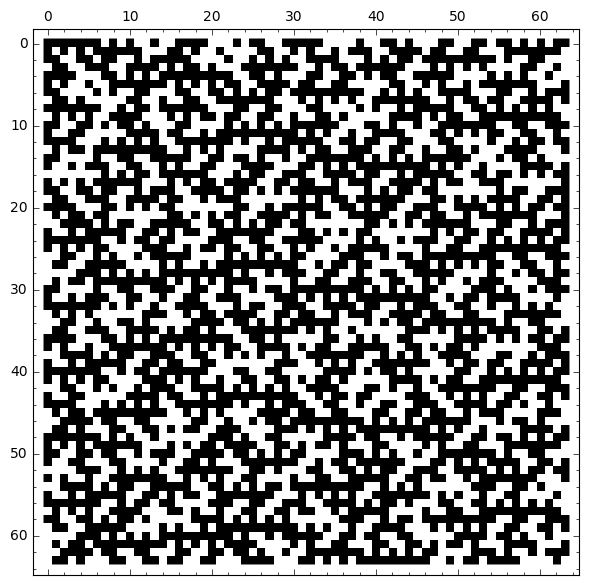
\includegraphics[width=.9\linewidth]{../matrix_plot/re6_4_weight_class_matrix.png}
  \captionof{figure}{$[f_{6,4}]$: weight classes}
  \label{fig:6_4_weight_class_matrix}
\end{minipage}%
\begin{minipage}{.48\textwidth}
  \centering
  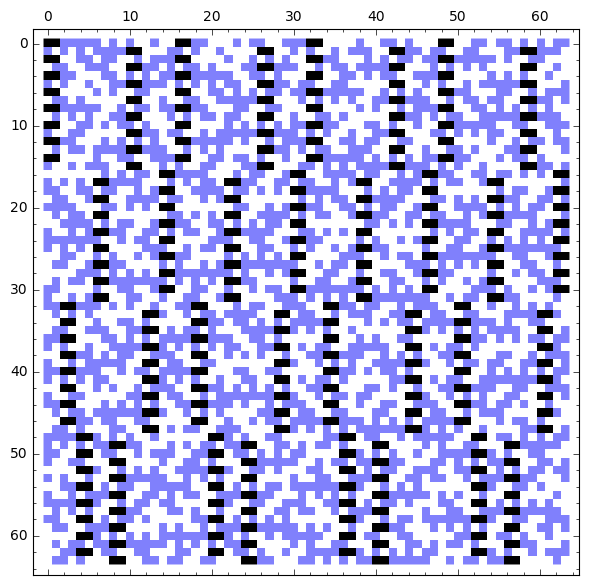
\includegraphics[width=.9\linewidth]{../matrix_plot/re6_4_bent_cayley_graph_index_matrix.png}
  \captionof{figure}{$[f_{6,4}]$: 3 extended Cayley classes}
  \label{fig:6_4_bent_cayley_graph_index_matrix}
\end{minipage}
\end{figure}
\end{frame}
\begin{colortheme}{seagull}
\begin{frame}
\frametitle{For 8 dimensions: \\ number of bent functions and EA classes}

According to Langevin and Leander (2011)
there are $99270589265934370305785861242880 \approx 2^{106}$ bent functions in dimension 8.

~

The number of EA classes has not yet been published, let alone a list of representatives.

\slidecite{Langevin and Leander 2011}
\end{frame}
\end{colortheme}
\begin{frame}
\frametitle{For 8 dimensions, up to degree 3: \\ extended translation classes}

Ten extended affine classes,

containing the following extended translation classes:

\tiny{}
\begin{align*}
\def\arraystretch{1.2}
\begin{array}{|cl|}
\hline
\text{Class} &
\text{Representative}
\\
\hline
\,[f_{ 8 , 1 }] & f_{ 8 , 1 } :=
\begin{array}{l}
x_{0} x_{1} + x_{2} x_{3} + x_{4} x_{5} + x_{6} x_{7}
\end{array}
\\
\,[f_{ 8 , 2 }] & f_{ 8 , 2 } :=
\begin{array}{l}
x_{0} x_{1} x_{2} + x_{0} x_{3} + x_{1} x_{4} + x_{2} x_{5} + x_{6} x_{7}
\end{array}
\\
\,[f_{ 8 , 3 }] & f_{ 8 , 3 } :=
\begin{array}{l}
x_{0} x_{1} x_{2} + x_{0} x_{6} + x_{1} x_{3} x_{4} + x_{1} x_{5} + x_{2} x_{3} + x_{4} x_{7}
\end{array}
\\
\,[f_{ 8 , 4 }] & f_{ 8 , 4 } :=
\begin{array}{l}
x_{0} x_{1} x_{2} + x_{0} x_{2} + x_{0} x_{4} + x_{1} x_{3} x_{4} + x_{1} x_{5} + x_{2} x_{3} + x_{6} x_{7}
\end{array}
\\
\,[f_{ 8 , 5 }] & f_{ 8 , 5 } :=
\begin{array}{l}
x_{0} x_{1} x_{2} + x_{0} x_{6} + x_{1} x_{3} x_{4} + x_{1} x_{4} + x_{1} x_{5} + x_{2} x_{3} x_{5} + x_{2} x_{4} + x_{3} x_{7}
\end{array}
\\
\,[f_{ 8 , 6 }] & f_{ 8 , 6 } :=
\begin{array}{l}
x_{0} x_{1} x_{2} + x_{0} x_{2} + x_{0} x_{3} + x_{1} x_{3} x_{4} + x_{1} x_{6} + x_{2} x_{3} x_{5} + x_{2} x_{4} + x_{5} x_{7}
\end{array}
\\
\,[f_{ 8 , 7 }] & f_{ 8 , 7 } :=
\begin{array}{l}
x_{0} x_{1} x_{2} + x_{0} x_{1} + x_{0} x_{2} + x_{0} x_{3} + x_{1} x_{3} x_{4} + x_{1} x_{4} + x_{1} x_{5} + x_{2} x_{3} x_{5}
\\
+\,  x_{2} x_{4} + x_{6} x_{7}
\end{array}
\\
\,[f_{ 8 , 8 }] & f_{ 8 , 8 } :=
\begin{array}{l}
x_{0} x_{1} x_{2} + x_{0} x_{5} + x_{1} x_{3} x_{4} + x_{1} x_{6} + x_{2} x_{3} x_{5} + x_{2} x_{4} + x_{3} x_{7}
\end{array}
\\
\,[f_{ 8 , 9 }] & f_{ 8 , 9 } :=
\begin{array}{l}
x_{0} x_{1} x_{6} + x_{0} x_{3} + x_{1} x_{4} + x_{2} x_{3} x_{6} + x_{2} x_{5} + x_{3} x_{4} + x_{4} x_{5} x_{6} + x_{6} x_{7}
\end{array}
\\
\,[f_{ 8 , 10 }] & f_{ 8 , 10 } :=
\begin{array}{l}
x_{0} x_{1} x_{2} + x_{0} x_{3} x_{6} + x_{0} x_{4} + x_{0} x_{5} + x_{1} x_{3} x_{4} + x_{1} x_{6} + x_{2} x_{3} x_{5} + x_{2} x_{4}
\\
+\,  x_{3} x_{7}
\end{array}
\\
\hline
\end{array}
\end{align*}
\normalsize{}
\end{frame}
\begin{frame}
\frametitle{For ET class $[f_{8,1}]$: matrices}
\begin{figure}
\centering
\begin{minipage}{.48\textwidth}
  \centering
  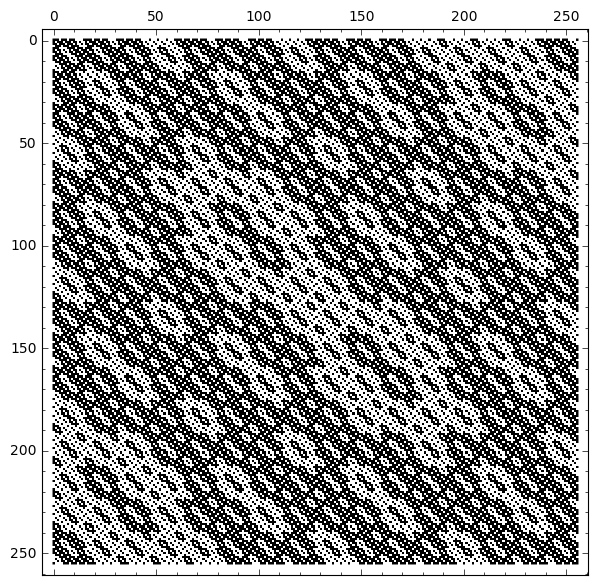
\includegraphics[width=.9\linewidth]{../matrix_plot/re8_1_weight_class_matrix.png}
  \captionof{figure}{$[f_{8,1}]$: weight classes}
  \label{fig:8_1_weight_class_matrix}
\end{minipage}%
\begin{minipage}{.48\textwidth}
  \centering
  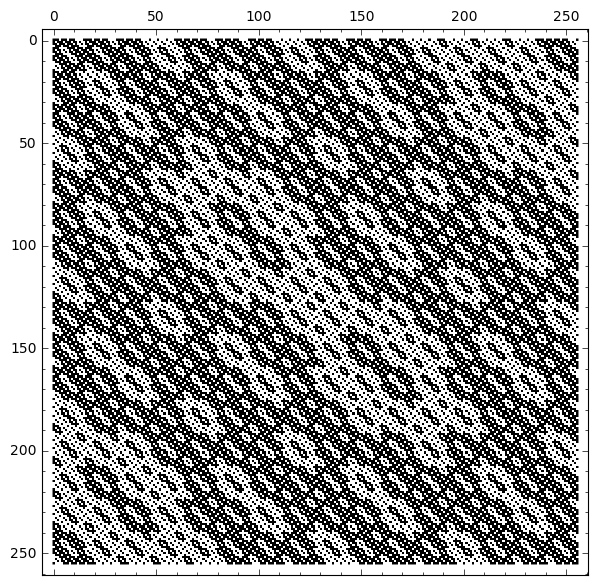
\includegraphics[width=.9\linewidth]{../matrix_plot/re8_1_bent_cayley_graph_index_matrix.png}
  \captionof{figure}{$[f_{8,1}]$: 2 extended Cayley classes}
  \label{fig:8_1_bent_cayley_graph_index_matrix}
\end{minipage}
\end{figure}
~
\end{frame}
\begin{frame}
\frametitle{For ET class $[f_{8,2}]$: matrices}
\begin{figure}
\centering
\begin{minipage}{.48\textwidth}
  \centering
  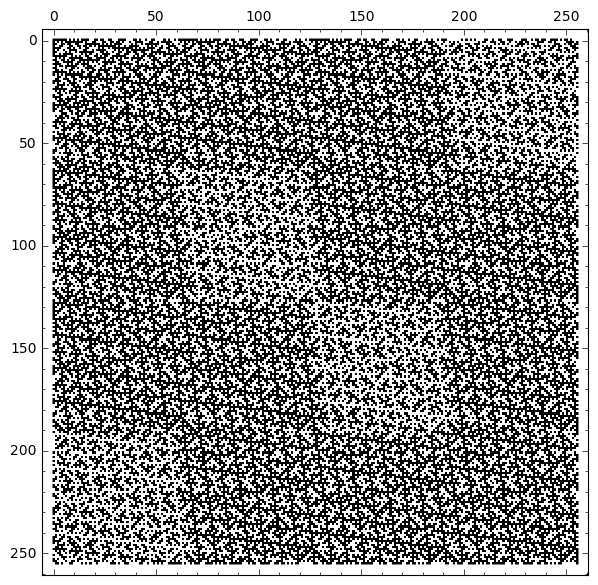
\includegraphics[width=.9\linewidth]{../matrix_plot/re8_2_weight_class_matrix.png}
  \captionof{figure}{$[f_{8,2}]$: weight classes}
  \label{fig:8_2_weight_class_matrix}
\end{minipage}%
\begin{minipage}{.48\textwidth}
  \centering
  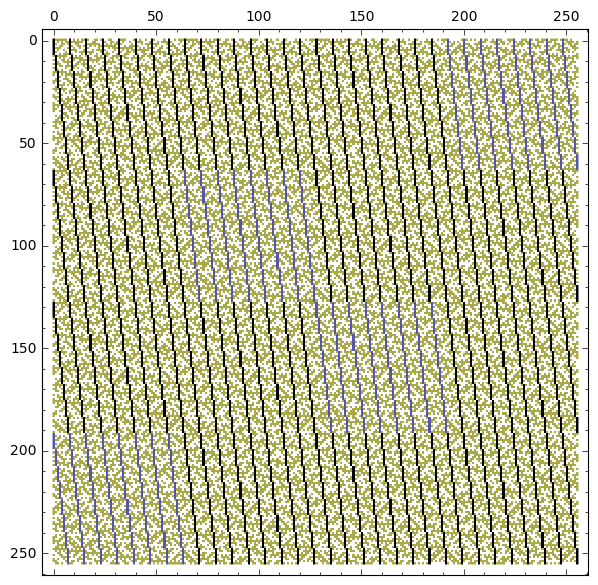
\includegraphics[width=.9\linewidth]{../matrix_plot/re8_2_bent_cayley_graph_index_matrix.png}
  \captionof{figure}{$[f_{8,2}]$: 4 extended Cayley classes}
  \label{fig:8_2_bent_cayley_graph_index_matrix}
\end{minipage}
\end{figure}
~
\end{frame}
\begin{frame}
\frametitle{For ET class $[f_{8,3}]$: matrices}
\begin{figure}
\centering
\begin{minipage}{.48\textwidth}
  \centering
  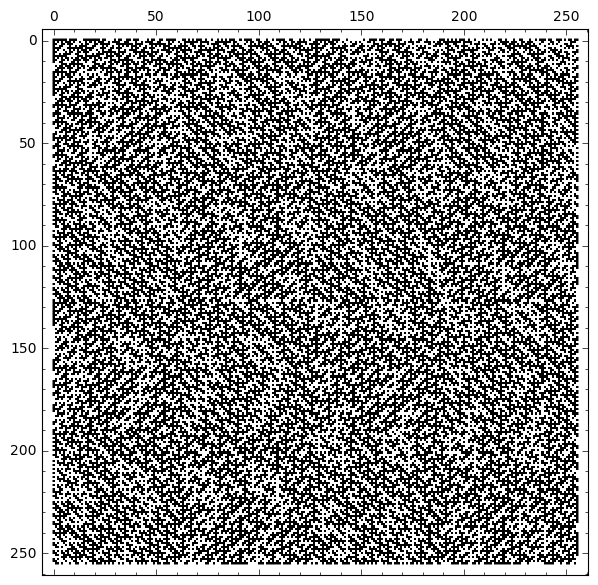
\includegraphics[width=.9\linewidth]{../matrix_plot/re8_3_weight_class_matrix.png}
  \captionof{figure}{$[f_{8,3}]$: weight classes}
  \label{fig:8_3_weight_class_matrix}
\end{minipage}%
\begin{minipage}{.48\textwidth}
  \centering
  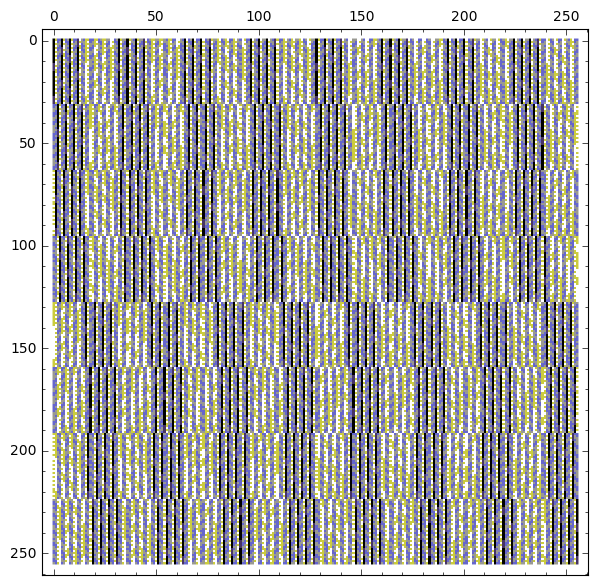
\includegraphics[width=.9\linewidth]{../matrix_plot/re8_3_bent_cayley_graph_index_matrix.png}
  \captionof{figure}{$[f_{8,3}]$: 6 extended Cayley classes}
  \label{fig:8_3_bent_cayley_graph_index_matrix}
\end{minipage}
\end{figure}
~
\end{frame}
\begin{frame}
\frametitle{For ET class $[f_{8,4}]$: matrices}
\begin{figure}
\centering
\begin{minipage}{.48\textwidth}
  \centering
  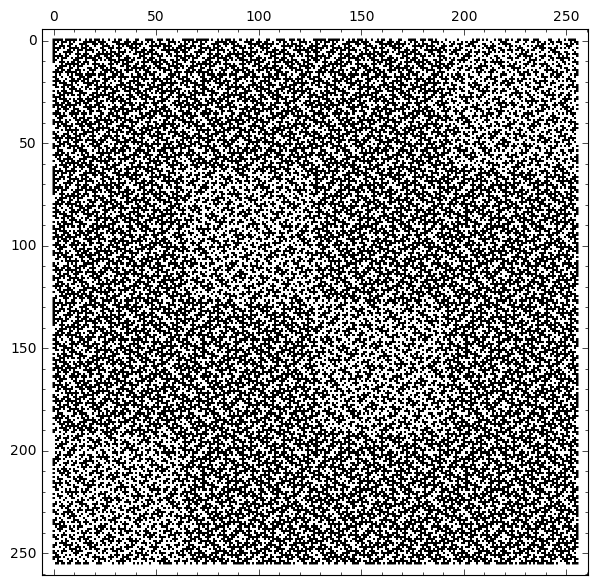
\includegraphics[width=.9\linewidth]{../matrix_plot/re8_4_weight_class_matrix.png}
  \captionof{figure}{$[f_{8,4}]$: weight classes}
  \label{fig:8_4_weight_class_matrix}
\end{minipage}%
\begin{minipage}{.48\textwidth}
  \centering
  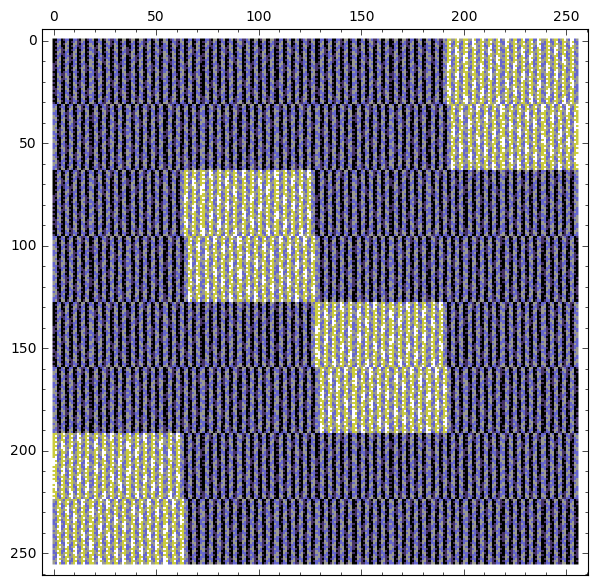
\includegraphics[width=.9\linewidth]{../matrix_plot/re8_4_bent_cayley_graph_index_matrix.png}
  \captionof{figure}{$[f_{8,4}]$: 5 extended Cayley classes}
  \label{fig:8_4_bent_cayley_graph_index_matrix}
\end{minipage}
\end{figure}
~
\end{frame}
\begin{frame}
\frametitle{For ET class $[f_{8,5}]$: matrices}
\begin{figure}
\centering
\begin{minipage}{.48\textwidth}
  \centering
  \includegraphics[width=.9\linewidth]{../matrix_plot/re8_5_weight_class_matrix.png}
  \captionof{figure}{$[f_{8,5}]$: weight classes}
  \label{fig:8_5_weight_class_matrix}
\end{minipage}%
\begin{minipage}{.48\textwidth}
  \centering
  \includegraphics[width=.9\linewidth]{../matrix_plot/re8_5_bent_cayley_graph_index_matrix.png}
  \captionof{figure}{$[f_{8,5}]$: 9 extended Cayley classes}
  \label{fig:8_5_bent_cayley_graph_index_matrix}
\end{minipage}
\end{figure}
~
\end{frame}
\begin{frame}
\frametitle{For ET class $[f_{8,6}]$: matrices}
\begin{figure}
\centering
\begin{minipage}{.48\textwidth}
  \centering
  \includegraphics[width=.9\linewidth]{../matrix_plot/re8_6_weight_class_matrix.png}
  \captionof{figure}{$[f_{8,6}]$: weight classes}
  \label{fig:8_6_weight_class_matrix}
\end{minipage}%
\begin{minipage}{.48\textwidth}
  \centering
  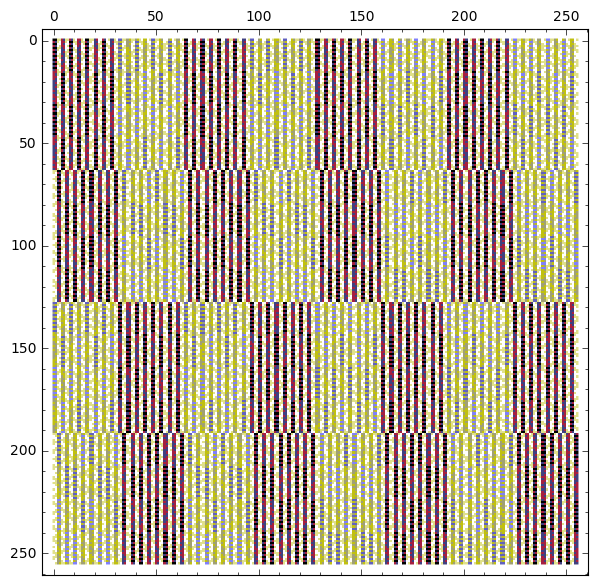
\includegraphics[width=.9\linewidth]{../matrix_plot/re8_6_bent_cayley_graph_index_matrix.png}
  \captionof{figure}{$[f_{8,6}]$: 9 extended Cayley classes}
  \label{fig:8_6_bent_cayley_graph_index_matrix}
\end{minipage}
\end{figure}
The same 9 classes as $[f_{8,5}]$, with the same frequencies!
\end{frame}
\begin{frame}
\frametitle{For ET class $[f_{8,7}]$: matrices}
\begin{figure}
\centering
\begin{minipage}{.48\textwidth}
  \centering
  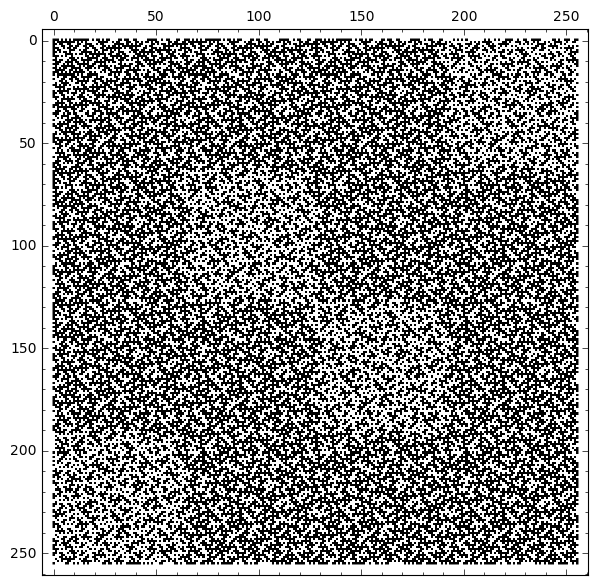
\includegraphics[width=.9\linewidth]{../matrix_plot/re8_7_weight_class_matrix.png}
  \captionof{figure}{$[f_{8,7}]$: weight classes}
  \label{fig:8_7_weight_class_matrix}
\end{minipage}%
\begin{minipage}{.48\textwidth}
  \centering
  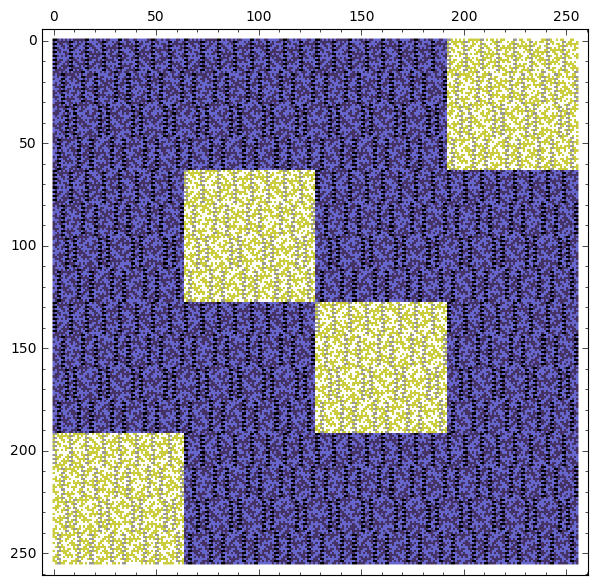
\includegraphics[width=.9\linewidth]{../matrix_plot/re8_7_bent_cayley_graph_index_matrix.png}
  \captionof{figure}{$[f_{8,7}]$: 5 extended Cayley classes}
  \label{fig:8_7_bent_cayley_graph_index_matrix}
\end{minipage}
\end{figure}
~
\end{frame}
\begin{frame}
\frametitle{For ET class $[f_{8,8}]$: matrices}
\begin{figure}
\centering
\begin{minipage}{.48\textwidth}
  \centering
  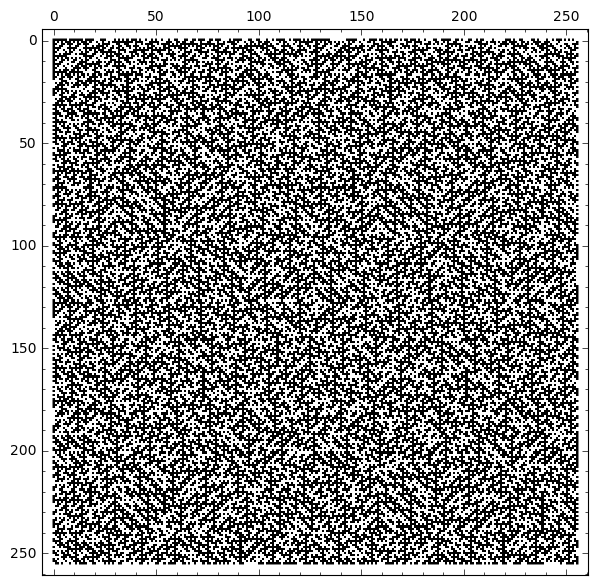
\includegraphics[width=.9\linewidth]{../matrix_plot/re8_8_weight_class_matrix.png}
  \captionof{figure}{$[f_{8,8}]$: weight classes}
  \label{fig:8_8_weight_class_matrix}
\end{minipage}%
\begin{minipage}{.48\textwidth}
  \centering
  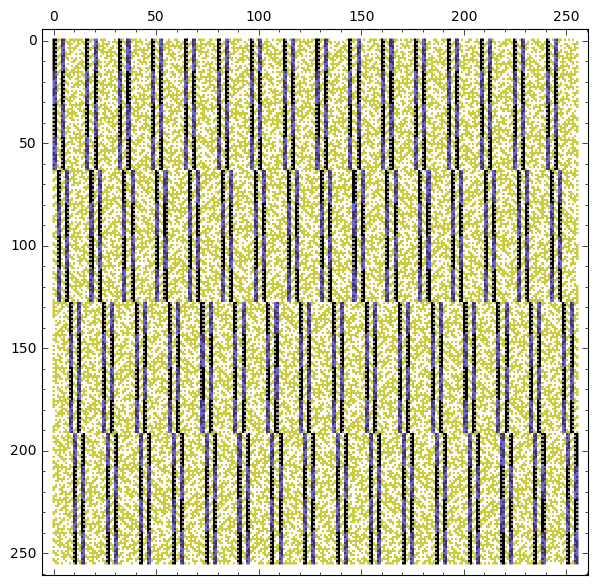
\includegraphics[width=.9\linewidth]{../matrix_plot/re8_8_bent_cayley_graph_index_matrix.png}
  \captionof{figure}{$[f_{8,8}]$: 6 extended Cayley classes}
  \label{fig:8_8_bent_cayley_graph_index_matrix}
\end{minipage}
\end{figure}
~
\end{frame}
\begin{frame}
\frametitle{For ET class $[f_{8,9}]$: matrices}
\begin{figure}
\centering
\begin{minipage}{.48\textwidth}
  \centering
  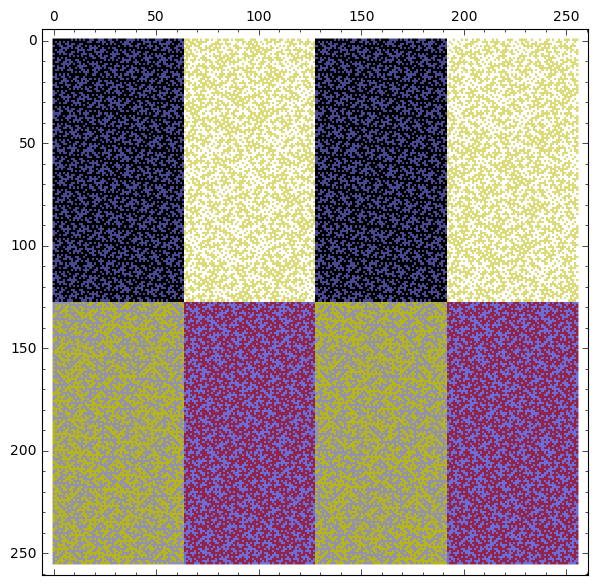
\includegraphics[width=.9\linewidth]{../matrix_plot/re8_9_bent_cayley_graph_index_matrix.png}
  \captionof{figure}{$[f_{8,9}]$: 8 extended Cayley classes ~~ ~~~~ ~~~~ ~~~~~~~~~}
  \label{fig:c8_9_bent_cayley_graph_index_matrix}
\end{minipage}
\begin{minipage}{.48\textwidth}
  \centering
  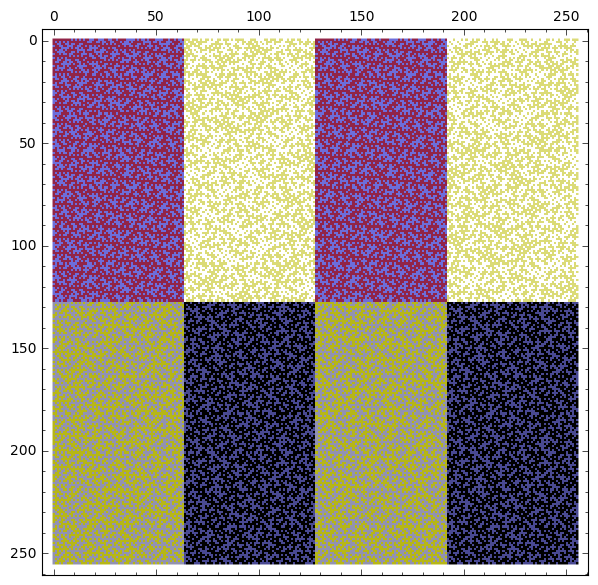
\includegraphics[width=.9\linewidth]{../matrix_plot/re8_9_dual_cayley_graph_index_matrix.png}
  \captionof{figure}{$[f_{8,9}]$: 8 extended Cayley classes of dual bent functions}
  \label{fig:c8_9_dual_cayley_graph_index_matrix}
\end{minipage}%
\end{figure}
4 of the 8 classes form 2 dual pairs of classes.
\end{frame}
\begin{frame}
\frametitle{For ET class $[f_{8,10}]$: matrices}
\begin{figure}
\centering
\begin{minipage}{.48\textwidth}
  \centering
  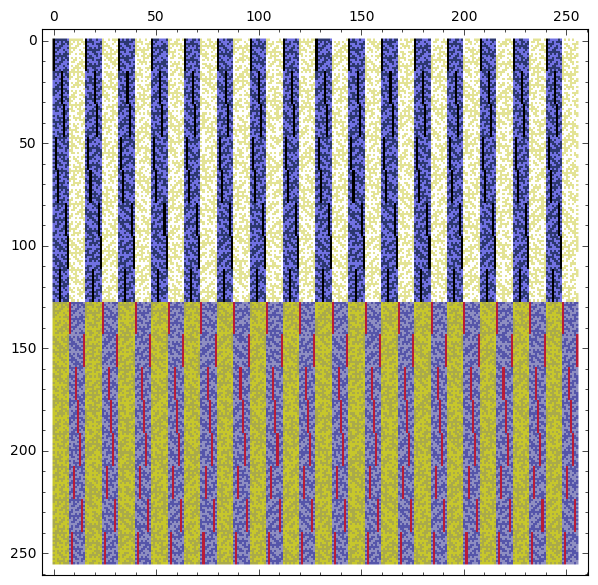
\includegraphics[width=.9\linewidth]{../matrix_plot/re8_10_bent_cayley_graph_index_matrix.png}
  \captionof{figure}{$[f_{8,10}]$: 10 extended Cayley classes ~~ ~~~~ ~~~~ ~~~~~~~~~}
  \label{fig:c8_10_bent_cayley_graph_index_matrix}
\end{minipage}
\begin{minipage}{.48\textwidth}
  \centering
  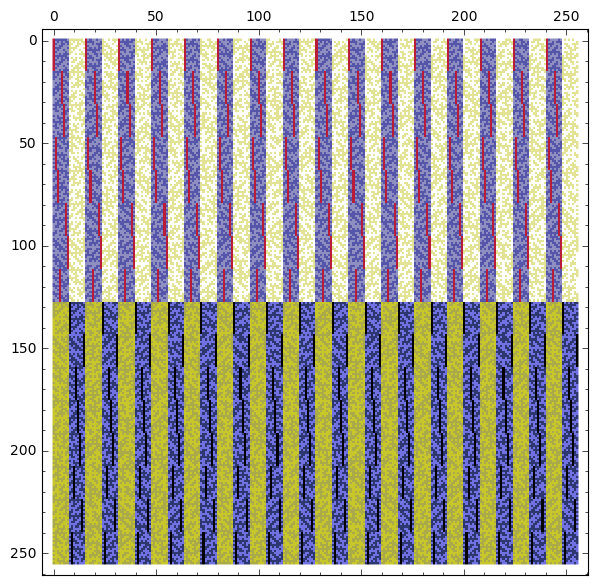
\includegraphics[width=.9\linewidth]{../matrix_plot/re8_10_dual_cayley_graph_index_matrix.png}
  \captionof{figure}{$[f_{8,10}]$: 10 extended Cayley classes of dual bent functions}
  \label{fig:c8_10_dual_cayley_graph_index_matrix}
\end{minipage}%
\end{figure}
6 of the 10 classes form 3 dual pairs of classes.
\end{frame}
\end{colortheme}
\begin{colortheme}{seagull}
\begin{frame}[fragile]
\frametitle{For 8 dimensions: number of partial spread \\ bent functions and EA classes}

According to Langevin and Hou (2011)
there are $70576747237594114392064 \approx 2^{75.9}$ \Emph{partial spread} bent functions in dimension 8,
contained in $14758$ EA classes, of which $14756$ have degree 4.

~

The EA class representatives are listed at Langevin's web site

\begin{verbatim}
http://langevin.univ-tln.fr/project/spread/psp.html
\end{verbatim}

\slidecite{Langevin and Hou 2011}
\end{frame}
\end{colortheme}
\begin{colortheme}{jubata}
\begin{frame}
\frametitle{Example partial spread ET class $[psf_{9,5438}]$}
\begin{figure}
\centering
\begin{minipage}{.48\textwidth}
  \centering
  \includegraphics[width=.9\linewidth]{../matrix_plot/psf_9_5438_bent_cayley_graph_index_matrix.png}
  \captionof{figure}{$[psf_{9,5438}]$: 16 extended Cayley classes ~~ ~~~~ ~~~~ ~~~~~~~~~}
  \label{fig:psf_9_5438_bent_cayley_graph_index_matrix}
\end{minipage}
\begin{minipage}{.48\textwidth}
  \centering
  \includegraphics[width=.9\linewidth]{../matrix_plot/psf_9_5438_dual_cayley_graph_index_matrix.png}
  \captionof{figure}{$[psf_{9,5438}]$: 16 extended Cayley classes of dual bent functions}
  \label{fig:psf_9_5438_dual_cayley_graph_index_matrix}
\end{minipage}%
\end{figure}
6 of the 16 classes form 3 dual pairs of classes.
\end{frame}
\section{Questions}
\begin{frame}
\frametitle{Open problems}
Settled only for dimension up to 6:
\begin{enumerate}
\item
How many EC classes are there for each dimension?
Are there ``Exponential numbers'' of classes?
\item
Which ET classes contain the maximum number of different EC classes?
\item
Which EC classes overlap more than one ET class?
\item
Which bent functions are extended affine equivalent to their dual?
\item
Which bent functions are Cayley equivalent to their dual?
\end{enumerate}
~

Also, what are the remaining EA and EC classes of binary bent functions of dimension 8 and degree 4?

~

\slidecite{Kantor 1983; Jungnickel and Tonchev 1991; Langevin and Leander 2008, 2011}
\end{frame}
\end{colortheme}
\section{Source code}
\begin{colortheme}{jubata}
\begin{frame}[fragile]
\frametitle{Source code on GitHub and SageMathCloud}
~

GitHub: Sage and Python source code

\begin{verbatim}
https://github.com/penguian/Boolean-Cayley-graphs
\end{verbatim}

~

SageMathCloud: Public worksheets, Sage and Python source code

\begin{verbatim}
http://tinyurl.com/Boolean-Cayley-graphs
\end{verbatim}

\end{frame}
\end{colortheme}
\section{Last}
\begin{colortheme}{jubata}
\begin{frame}
\frametitle{Thank you.}

\begin{figure}
\centering
\begin{minipage}{.48\textwidth}
  \centering
  \includegraphics[width=.9\linewidth]{../matrix_plot/tau_3_bent_cayley_graph_index_matrix.png}
  \captionof{figure}{$[\tau_3]$: 3 extended Cayley classes}
  \label{fig:tau_3_bent_cayley_graph_index_matrix}
\end{minipage}
\begin{minipage}{.48\textwidth}
  \centering
  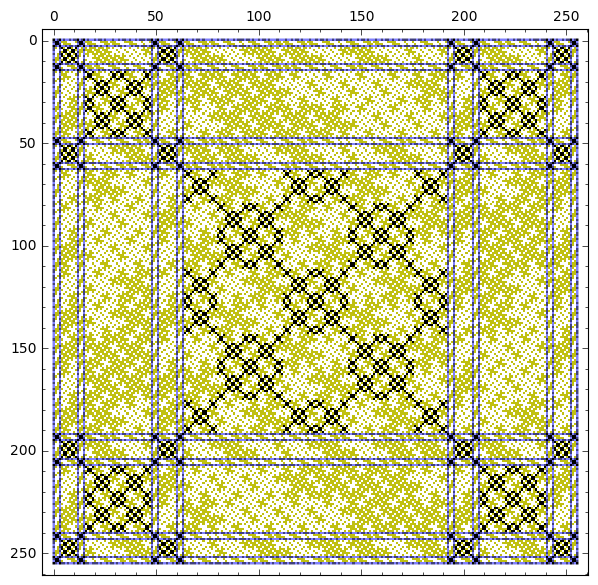
\includegraphics[width=.9\linewidth]{../matrix_plot/tau_4_bent_cayley_graph_index_matrix.png}
  \captionof{figure}{$[\tau_4]$: 5 extended Cayley classes}
  \label{fig:tau_4_bent_cayley_graph_index_matrix}
\end{minipage}%
\end{figure}
\end{frame}

\end{colortheme}
\end{document}
